\documentclass[tikz]{standalone}
\usepackage{tikz}
\usetikzlibrary{arrows.meta, positioning, decorations.pathmorphing, decorations.markings, calc, shapes.geometric, fit, matrix}
\usepackage{amsmath,amssymb}

\definecolor{DarkSkyBlue}{RGB}{0, 51, 153}
\definecolor{domain1}{RGB}{180, 220, 255}
\definecolor{domain2}{RGB}{255, 220, 180}
\definecolor{domain3}{RGB}{180, 255, 220}
\definecolor{domain4}{RGB}{220, 180, 255}
\definecolor{elderpurple}{RGB}{160, 120, 200}

\begin{document}

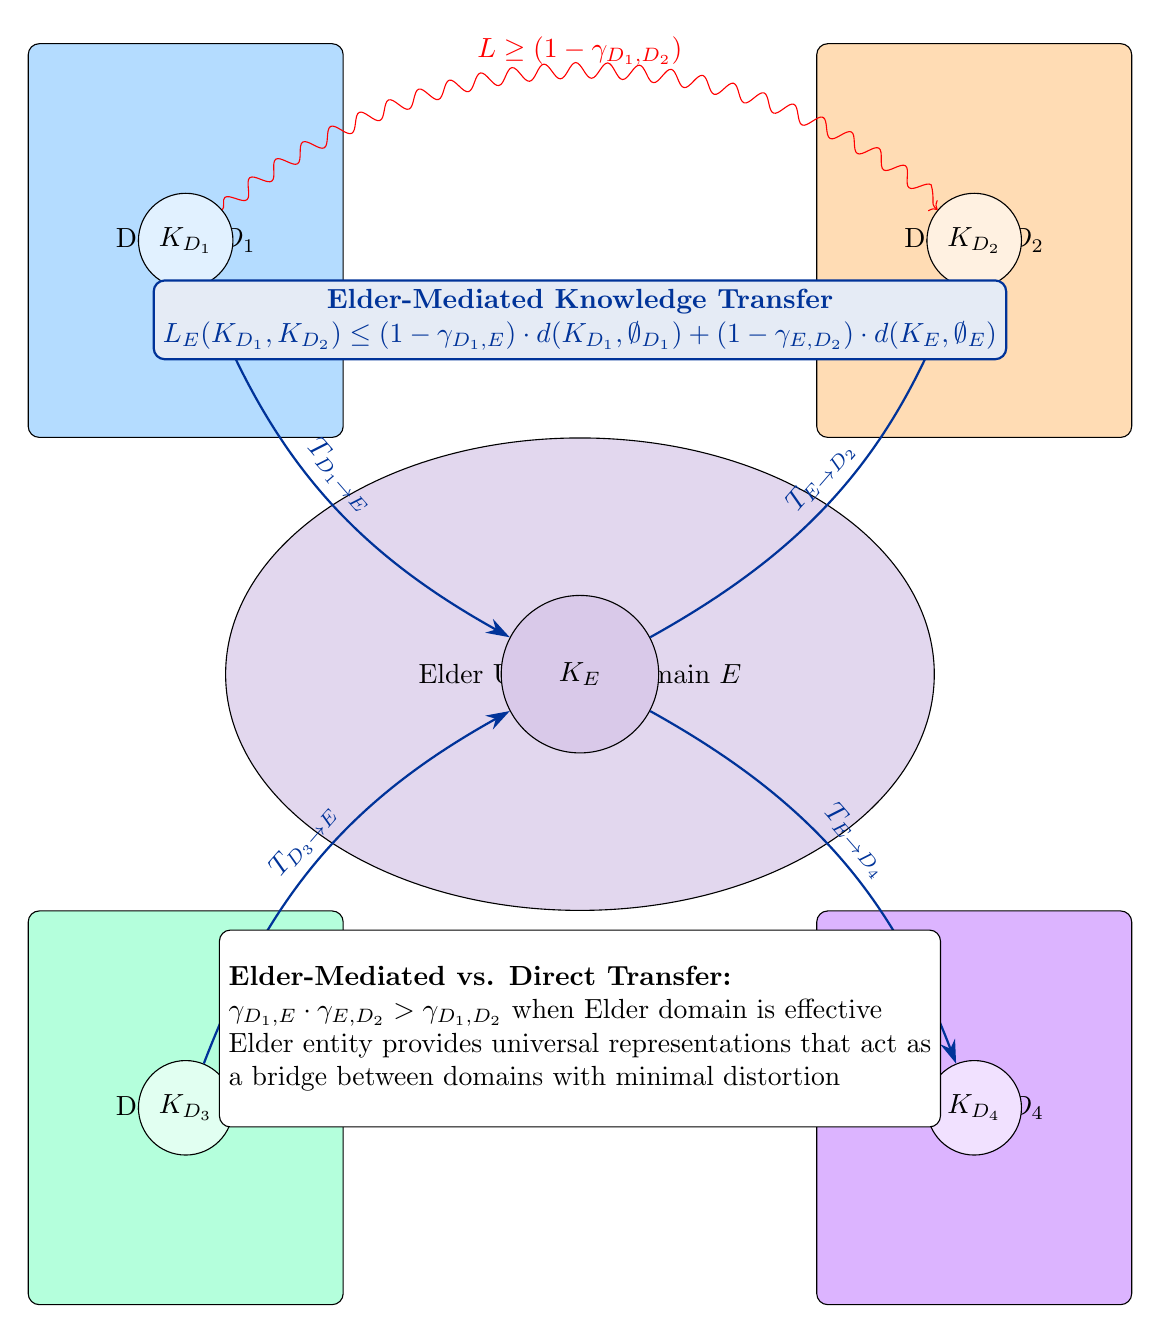
\begin{tikzpicture}[
    node distance=2.5cm,
    knowledge/.style={circle, draw, fill=white, minimum size=1.2cm, align=center},
    domain/.style={draw, rounded corners, minimum width=4cm, minimum height=5cm, align=center},
    arrow/.style={-{Stealth[length=3mm, width=2mm]}, line width=0.7pt},
    iso/.style={-{Stealth[length=3mm, width=2mm]}, DarkSkyBlue, line width=1pt},
    dasharrow/.style={dashed, ->, line width=0.5pt},
    elder_domain/.style={draw, fill=elderpurple!30, ellipse, minimum width=9cm, minimum height=6cm, align=center},
    distortion/.style={decorate, decoration={snake, amplitude=1mm, segment length=4mm}}
]

% Elder domain
\node[elder_domain] (elder) {Elder Universal Domain $E$};

% Domains
\node[draw, rounded corners, fill=domain1, minimum width=4cm, minimum height=5cm, align=center, above left=3cm and 3cm of elder.center] (d1) {Domain $D_1$};
\node[draw, rounded corners, fill=domain2, minimum width=4cm, minimum height=5cm, align=center, above right=3cm and 3cm of elder.center] (d2) {Domain $D_2$};
\node[draw, rounded corners, fill=domain3, minimum width=4cm, minimum height=5cm, align=center, below left=3cm and 3cm of elder.center] (d3) {Domain $D_3$};
\node[draw, rounded corners, fill=domain4, minimum width=4cm, minimum height=5cm, align=center, below right=3cm and 3cm of elder.center] (d4) {Domain $D_4$};

% Knowledge states
\node[knowledge, fill=domain1!40!white] (k1) at ($(d1) + (0,0)$) {$K_{D_1}$};
\node[knowledge, fill=domain2!40!white] (k2) at ($(d2) + (0,0)$) {$K_{D_2}$};
\node[knowledge, fill=domain3!40!white] (k3) at ($(d3) + (0,0)$) {$K_{D_3}$};
\node[knowledge, fill=domain4!40!white] (k4) at ($(d4) + (0,0)$) {$K_{D_4}$};

% Elder knowledge
\node[knowledge, fill=elderpurple!40!white, minimum size=2cm] (ke) at ($(elder)$) {$K_E$};

% Transfer paths
\draw[iso, thick] (k1) to[bend right=20] node[midway, above, sloped, text=DarkSkyBlue] {$T_{D_1 \to E}$} (ke);
\draw[iso, thick] (k3) to[bend left=20] node[midway, above, sloped, text=DarkSkyBlue] {$T_{D_3 \to E}$} (ke);
\draw[iso, thick] (ke) to[bend right=20] node[midway, above, sloped, text=DarkSkyBlue] {$T_{E \to D_2}$} (k2);
\draw[iso, thick] (ke) to[bend left=20] node[midway, above, sloped, text=DarkSkyBlue] {$T_{E \to D_4}$} (k4);

% Direct transfer (suboptimal)
\draw[distortion, red, ->] (k1) to[bend left=40] node[midway, above, text=red] {$L \geq (1 - \gamma_{D_1,D_2})$} (k2);

% Title
\node[rectangle, draw, DarkSkyBlue, thick, rounded corners, fill=white!90!DarkSkyBlue, minimum width=10cm, align=center] 
    at ($(d1)!0.5!(d4) + (0,4.5)$) {
    \textbf{Elder-Mediated Knowledge Transfer}\\
    $L_E(K_{D_1}, K_{D_2}) \leq (1 - \gamma_{D_1,E}) \cdot d(K_{D_1}, \emptyset_{D_1}) + (1 - \gamma_{E,D_2}) \cdot d(K_E, \emptyset_E)$
};

% Legend
\node[rectangle, draw, rounded corners, fill=white, minimum width=8cm, minimum height=2.5cm, align=left] 
    at ($(d1)!0.5!(d4) + (0,-4.5)$) {
    \textbf{Elder-Mediated vs. Direct Transfer:}\\
    $\gamma_{D_1,E} \cdot \gamma_{E,D_2} > \gamma_{D_1,D_2}$ when Elder domain is effective\\
    Elder entity provides universal representations that act as\\
    a bridge between domains with minimal distortion
};

\end{tikzpicture}

\end{document}